% Insert in the group's Results and Analysis section after Tasks 1 and 2.
% Requires amsmath and graphicx in the main document's preamble.
% Upload both referenced PNGs to the figures/ directory in Overleaf.
% Include the AI acknowledgment below in the group's final disclosure.

\subsection{Task 3 --- Simulating the original random walk}
\label{subsec:atp-original-walk}

We simulated the walk on the completed transition matrix \(P\).
The row vector \(x_k\) gives the probabilities after \(k\) steps.
In each run we placed all the initial probability on one player.
Djokovic (ID 130) starts in the largest original strongly connected
component and gives \(1/51\) to each player who beat him on his first move.
Bopanna (ID 8) has no outgoing match arrows, so his first step gives
every player probability \(1/1191\).

We used NumPy to apply \(x_k=x_{k-1}P\), which gives \(x_k=x_0P^k\)
after \(k\) moves. We recorded each vector and its change,
\[
\Delta_k=\lVert x_k-x_{k-1}\rVert_1
=\sum_{j=1}^{1191}\left|(x_k)_j-(x_{k-1})_j\right|.
\]
Absolute values prevent gains and losses at different players from
cancelling. We stopped at the first \(\Delta_k<10^{-10}\) or after 5,000
updates. The function returned the last vector, update count, distribution
and change histories, and whether the threshold was reached. We checked
that all saved distributions had nonnegative entries summing to one.

\begin{table}[htbp]
  \centering
  \caption{Stopping results for the completed original walk.}
  \label{tab:atp-original-stopping}
  \begin{tabular}{lrrl}
    \hline
    Starting player & Updates & Last \(\Delta_k\) & Threshold reached \\
    \hline
    Novak Djokovic & 28 & \(6.628\times 10^{-11}\) & Yes \\
    Rohan Bopanna & 33 & \(7.305\times 10^{-11}\) & Yes \\
    \hline
  \end{tabular}
\end{table}

The early trajectories differ because Bopanna immediately spreads
probability across the full graph, while Djokovic initially reaches only
his direct opponents. Figure~\ref{fig:atp-original-trajectories} shows
the two starts alongside Zverev, our predicted leader, and Damm, a
lower-ranked player. The plotted probabilities settle at the same levels
and the final vectors differ by only \(7.797\times10^{-11}\) in \(L^1\).
Figure~\ref{fig:atp-original-convergence} shows both runs crossing the
threshold. We observed no sustained oscillation.

\begin{figure}[htbp]
  \centering
  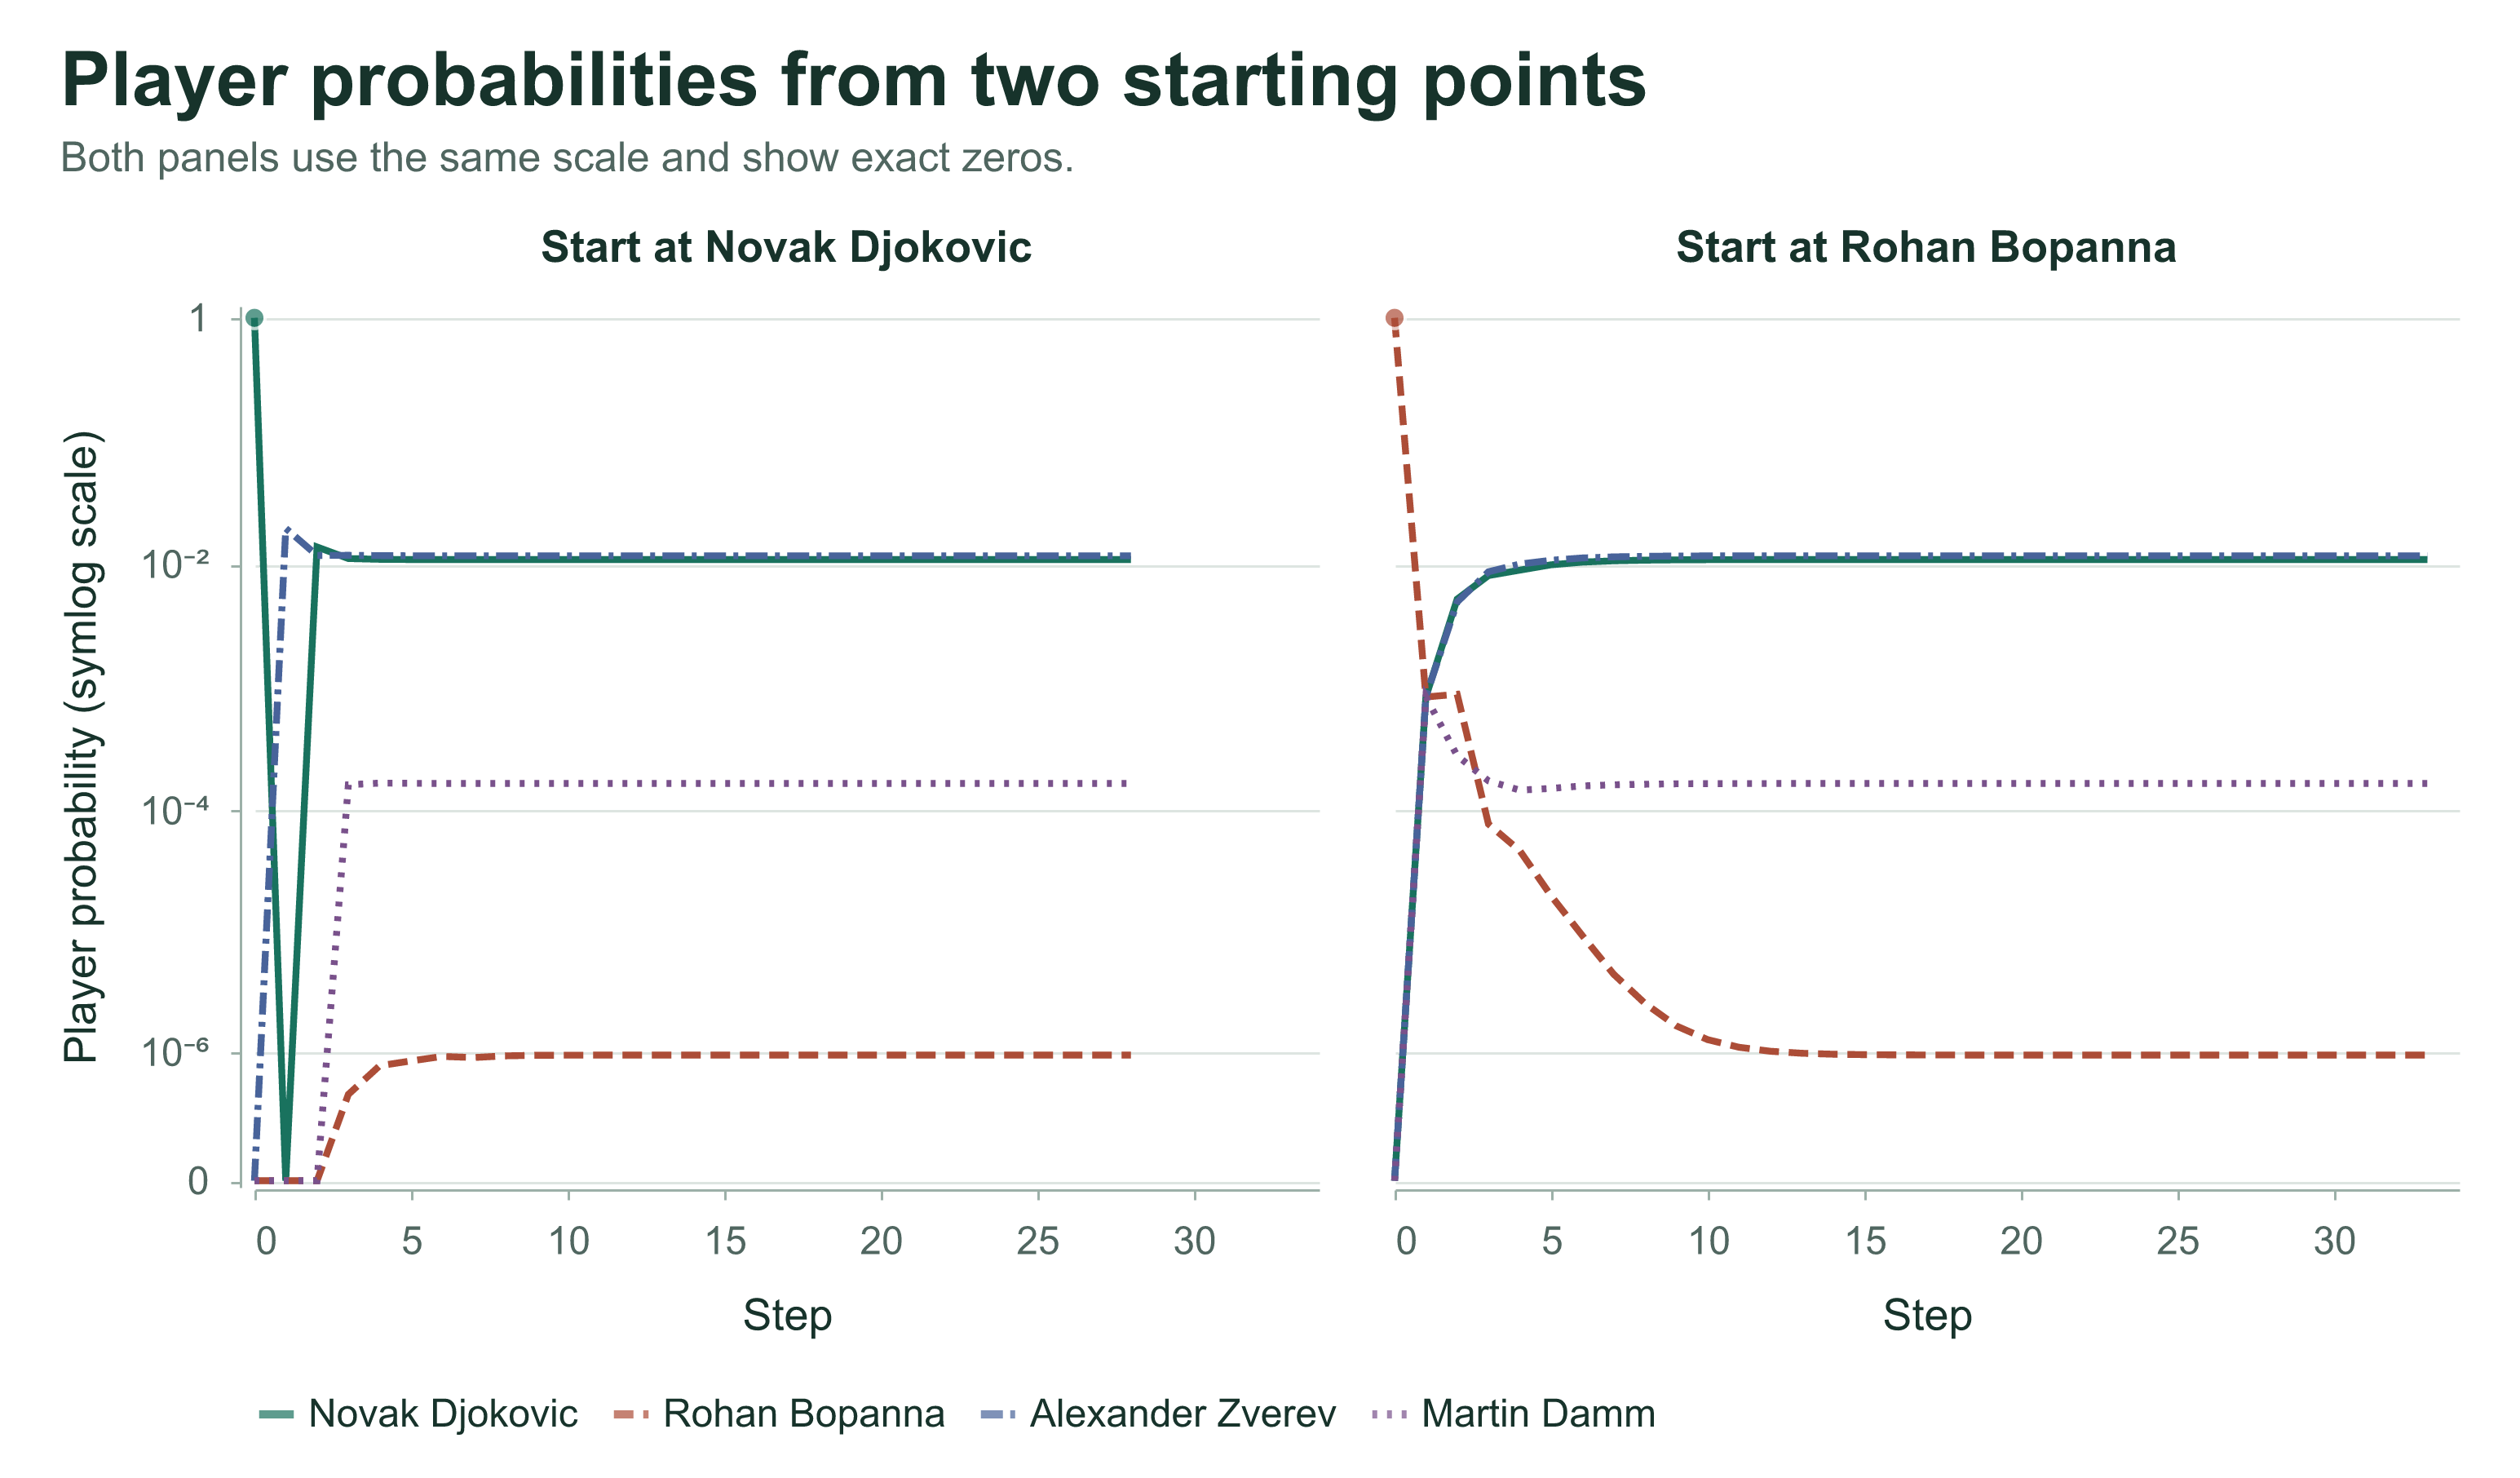
\includegraphics[width=\linewidth]{figures/task3_player_probabilities.png}
  \caption{Probability histories for selected players from the Djokovic and
  Bopanna starts. Both panels use a symmetric logarithmic scale, so exact zeros are visible alongside small positive probabilities.}
  \label{fig:atp-original-trajectories}
\end{figure}

\begin{figure}[htbp]
  \centering
  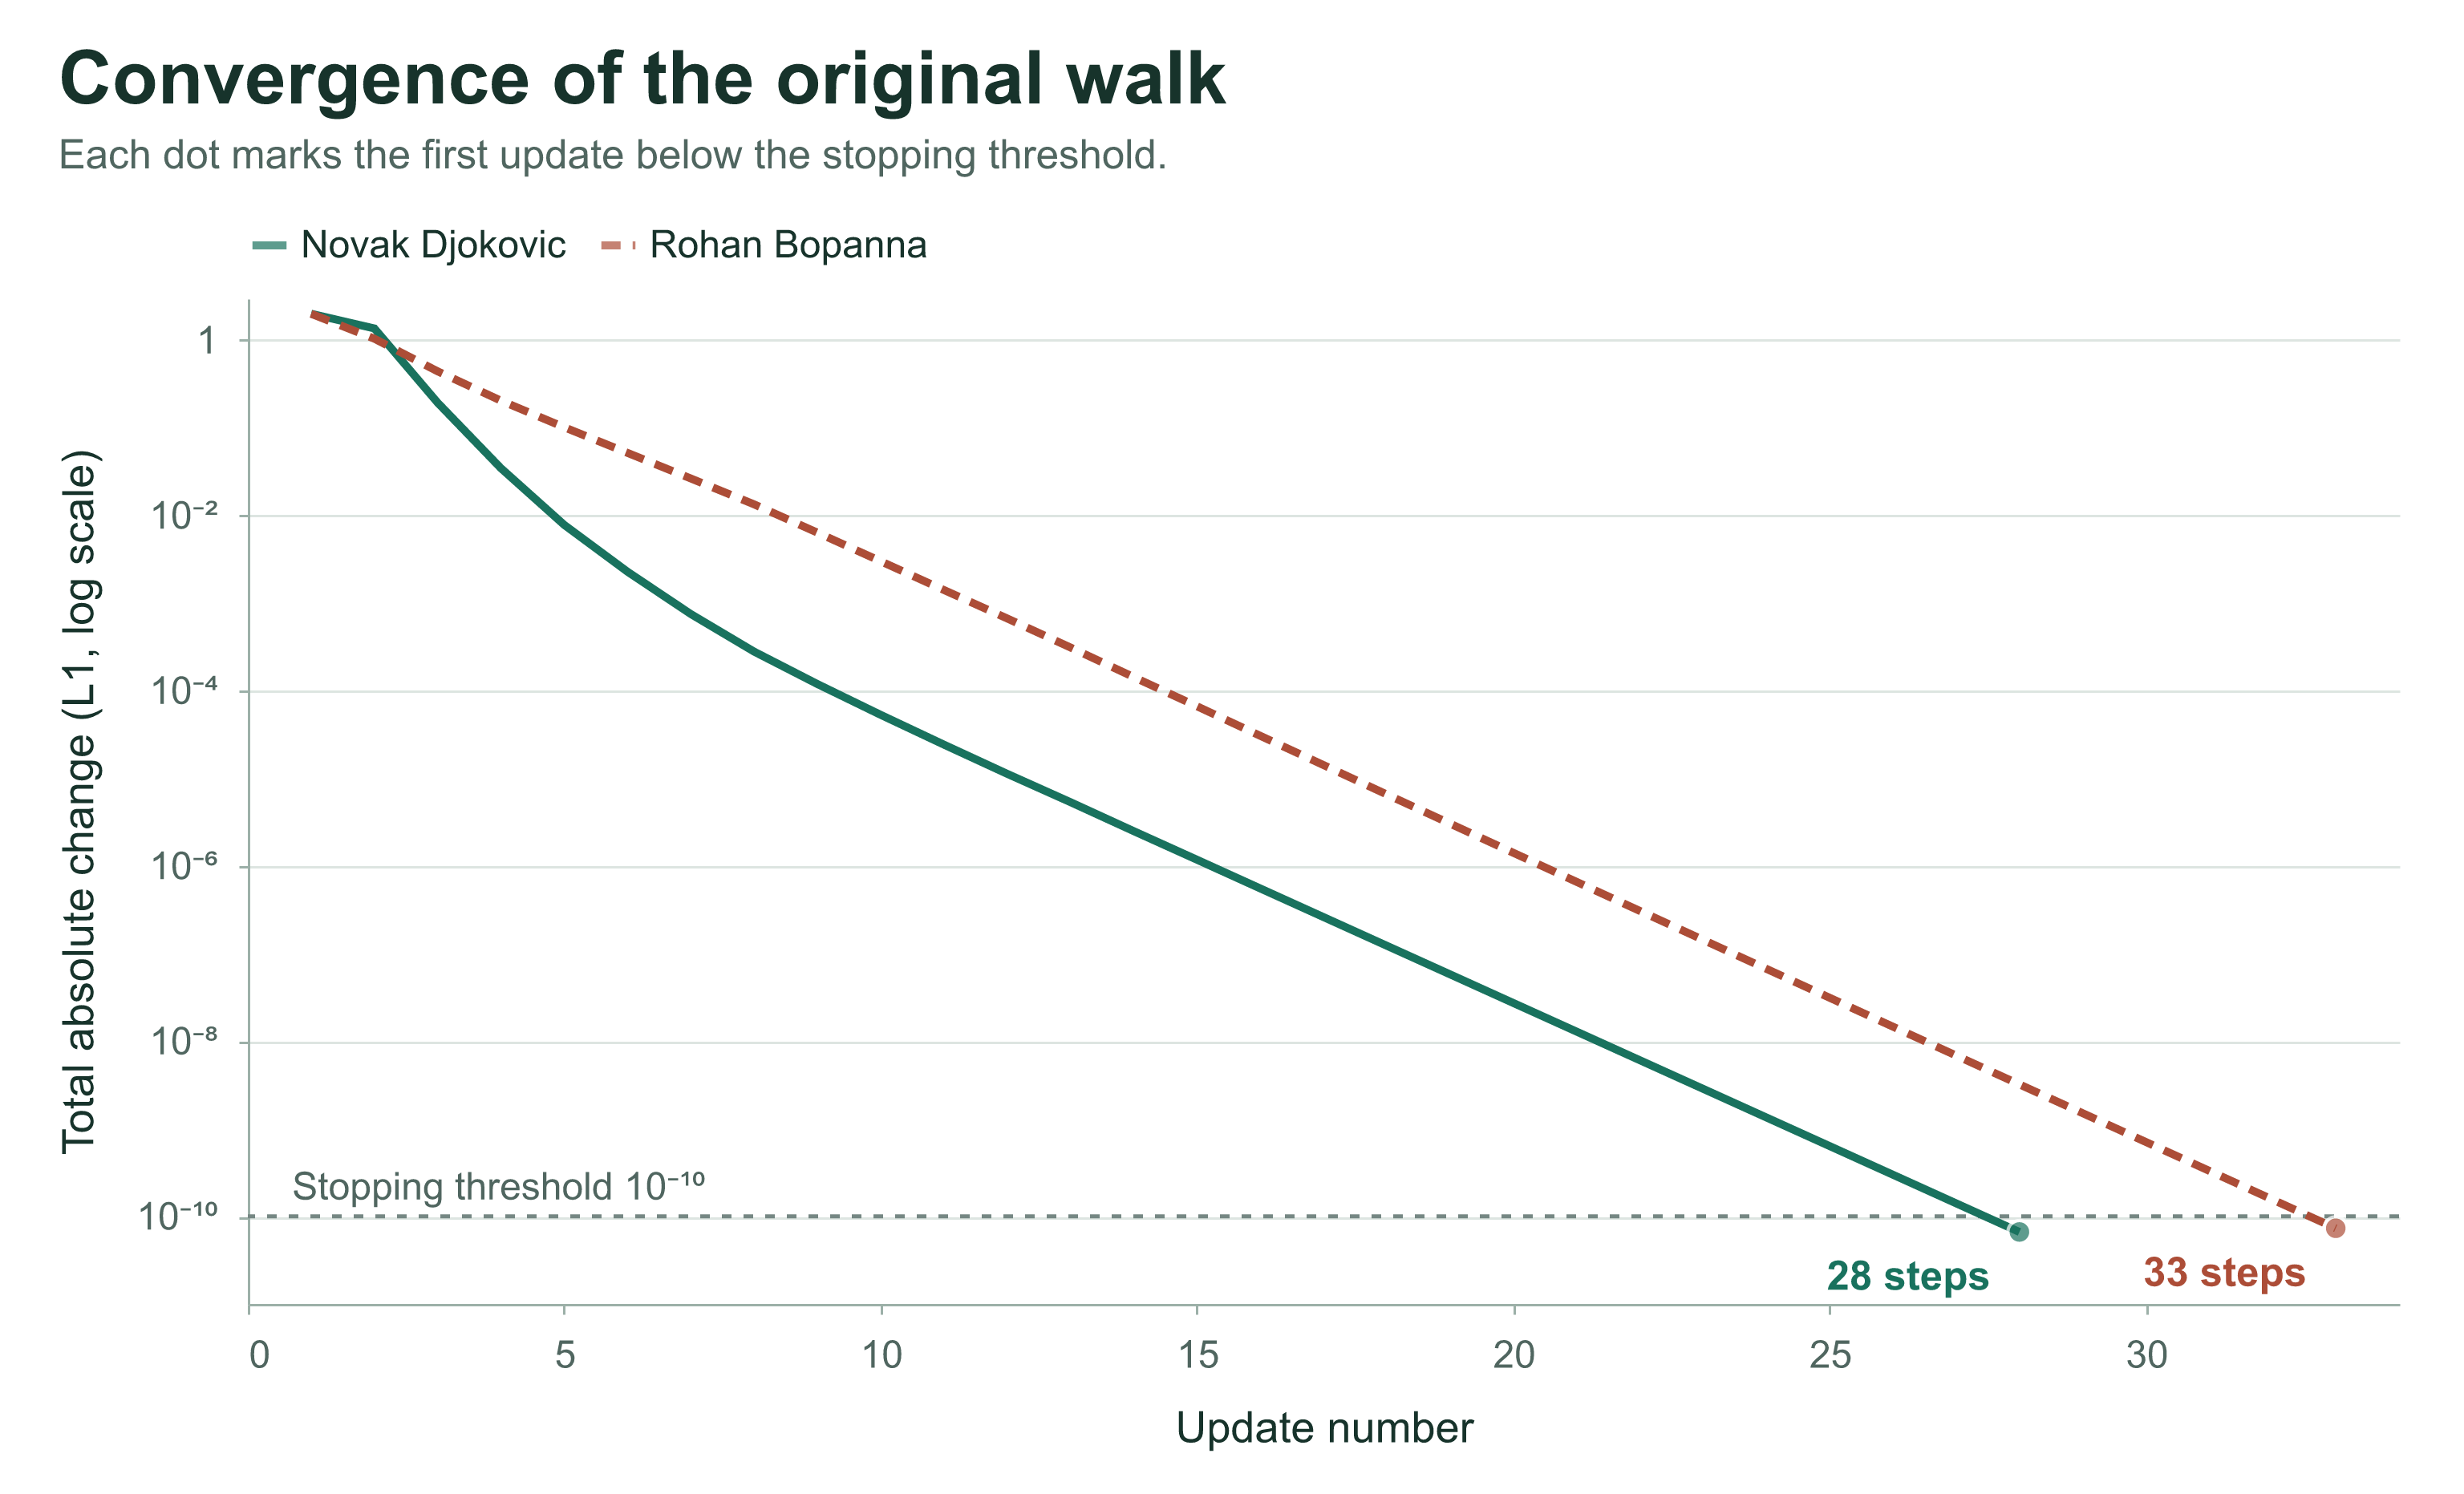
\includegraphics[width=0.69\linewidth]{figures/task3_convergence.png}
  \caption{Total absolute change between successive distributions.
  The horizontal dashed line shows the tolerance \(10^{-10}\). The labelled dots mark the first update below it.}
  \label{fig:atp-original-convergence}
\end{figure}

\subsection{Task 4 --- Stationary distribution and eigenvalues}
\label{subsec:atp-stationary}

A distribution \(\pi\) is stationary if \(\pi P=\pi\), so
one step leaves the probability on each player unchanged. Since \(\pi\)
is a row vector, we transpose to obtain
\(P^{\mathsf T}\pi^{\mathsf T}=1\cdot\pi^{\mathsf T}\), the right
eigenvector equation used by \texttt{numpy.linalg.eig(P.T)}.
We found the real eigenvector at \(1\) and divided by the sum of its
entries to fix its scale and sign. The normalized entries sum to \(1\)
and the smallest is \(4.7302\times10^{-7}\).
The residual \(\lVert\pi P-\pi\rVert_1\) was \(7.752\times10^{-16}\).
The final Djokovic and Bopanna vectors differed from \(\pi\) by
\(5.901\times10^{-11}\) and \(6.495\times10^{-11}\) in \(L^1\).
Zverev ranked first at \(1.1736\%\) of the long-run probability, supporting
our Task~2 prediction. This score depends on the binary match links, which
collapse repeated wins and omit factors such as court surface.

\subsubsection*{Two stationary equations worked out by hand}

For a target player \(j\), we expand \(\pi_j=\sum_i\pi_iP_{ij}\) by
adding all incoming contributions. A non-dangling source \(i\) contributes
\(\pi_i/d_i\) along each of its \(d_i\) outgoing arrows. Every dangling
source contributes \(\pi_i/1191\) to each destination. The combined
contribution from the 63 dangling sources to any one destination is
\[
c=\frac{1}{1191}\sum_{i:\,d_i=0}\pi_i
\approx 4.73020165\times10^{-7}.
\]

\paragraph{Rohan Bopanna (ID 8).}
Hong Chung (ID 370) is his only incoming match source. Hong Chung has
out-degree one, so Bopanna receives all of his probability along that arrow.
Adding the uniform contribution gives
\[
\begin{aligned}
\pi_{\text{Bopanna}}
&=\frac{\pi_{\text{Hong Chung}}}{1}+c\\
&\approx 4.73020165\times10^{-7}+4.73020165\times10^{-7}\\
&\approx 9.46040329\times10^{-7}.
\end{aligned}
\]

\paragraph{Martin Damm (ID 1).}
Damm receives match contributions from Zhizhen Zhang (ID 473),
Tommy Paul (ID 587), and Darwin Blanch (ID 1096), whose out-degrees
are 56, 76, and 4, respectively.
\[
\begin{aligned}
\pi_{\text{Damm}}
&=\frac{\pi_{\text{Zhang}}}{56}+\frac{\pi_{\text{Paul}}}{76}
  +\frac{\pi_{\text{Blanch}}}{4}+c\\
&\approx 4.60149237\times10^{-5}+1.02494447\times10^{-4}
  +1.78573641\times10^{-5}+4.73020165\times10^{-7}\\
&\approx 1.66839755\times10^{-4}.
\end{aligned}
\]
Both expanded equations reproduce the corresponding eigenvector entries
within rounding error.

\subsubsection*{Uniqueness and convergence}

All 63 original closed components are single dangling players.
The uniform rows allow the completed walk to leave them. By searching the
positive entries of \(P\) and then reversing the arrows, we verified that
Djokovic can reach all 1,191 players and all 1,191 can reach Djokovic.
Thus every player can reach every other via Djokovic. The completed chain
has one closed communicating class, and finite irreducibility gives a
unique stationary distribution.

We also verified two- and three-step returns to Djokovic via Nadal and
via Zverev and Federer, respectively. Since the greatest common divisor of
2 and 3 is 1, the completed chain is aperiodic. Irreducibility and
aperiodicity together explain why every initial distribution converges
to \(\pi\). Eigenvalues provide a separate numerical check. \(P\) and
\(P^{\mathsf T}\) share the same eigenvalues. One equals \(1\), and the
largest remaining magnitude is \(0.46953840\) from the pair
\(0.46951796\pm0.00438091\,\mathrm{i}\). The other modes therefore decay.
An eigenvalue of \(-1\) could sustain alternation, and we found none
near \(-1\), in line with the Task~3 runs.

% Suggested AI disclosure for this section: We used OpenAI Codex to assist
% with the Python implementation, numerical verification, figure generation,
% and wording of the methods and results for Tasks 3 and 4.
